\documentclass[a4paper,10pt]{article}
\usepackage{tikz}
\usepackage[utf8]{inputenc}
\usepackage{listings}
% Er zijn talloze parameters ...
\lstset{language=C++, showstringspaces=false, basicstyle=\small,
  numbers=left, numberstyle=\tiny, numberfirstline=false,
  stepnumber=1, tabsize=8, 
  commentstyle=\ttfamily, identifierstyle=\ttfamily,
  stringstyle=\itshape}
\usepackage{amsmath}

%opening
\title{ Hogebomen }
\author{ Lisette de Schipper (s1396250) en Micky Faas (s1407937) }
\date{}

\begin{document}

\maketitle

\begin{abstract}
Blabla
\end{abstract}

\section{Inleiding}
AVL-bomen, splay-bomen en treaps zijn klassieke datastructuren die ingezet worden om een verzameling gegevens te faciliteren. Het zijn zelfbalancerende binaire zoekbomen die elk een vorm van ruimte en/of tijd-effici\"entie aanbieden. Er worden experimenten verricht om de prestatie van deze zelf-balancerende zoekbomen te vergelijken, aan de hand van ophaaltijd van data, mate van herstructurering en het verwijderen van knopen. Ook wordt de prestatie van deze zoekbomen uitgezet tegen de ongebalanceerde tegenhanger, de binaire zoekboom.

\section{Werkwijze}
De vier bomen zijn conceptueel eenvoudig en relatief makkelijk te implementeren.
\subsection{Implementatie binaire zoekboom}
TO DO
\subsection{Implementatie AVL-bomen}
Knopen van een AVL-boom hebben een \emph{balansfactor}, die altijd -1, 0 of 1 moet zijn. In deze implementatie is de balansfactor de hoogte van de rechtersubboom min de hoogte van de linkersubboom. Dit houdt dus in dat de hoogte van de linkersubboom van de wortel met maar 1 knoop kan verschillen van de hoogte van de rechtersubboom van de wortel. Het moment dat de balansfactor van een knoop minder dan -1 of meer dan 1 wordt, moet de boom geherstructureerd worden, om deze eigenschap te herstellen. \\

Om de balansfactor voor elke knoop te berekenen, houdt elke knoop zijn eigen hoogte bij. De balansfactor van een knoop wordt hersteld door rotaties. De richting en de hoeveelheid van de rotaties hangt af van de vorm van de betreffende (sub)boom. De volgende twee vormen en hun spiegelbeelden kunnen voorkomen bij het verwijderen of toevoegen van een knoop: \\

\begin{center}
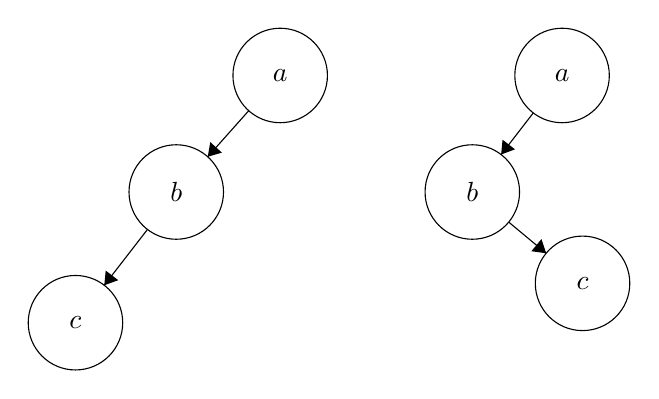
\begin{tikzpicture}[scale=0.2]
\tikzstyle{every node}+=[inner sep=0pt]
\draw [black] (16.5,-14.5) circle (3);
\draw (16.5,-14.5) node {$a$};
\draw [black] (9.9,-21.9) circle (3);
\draw (9.9,-21.9) node {$b$};
\draw [black] (34.4,-14.5) circle (3);
\draw (34.4,-14.5) node {$a$};
\draw [black] (3.5,-30.2) circle (3);
\draw (3.5,-30.2) node {$c$};
\draw [black] (28.7,-21.9) circle (3);
\draw (28.7,-21.9) node {$b$};
\draw [black] (35.7,-27.7) circle (3);
\draw (35.7,-27.7) node {$c$};
\draw [black] (14.5,-16.74) -- (11.9,-19.66);
\fill [black] (11.9,-19.66) -- (12.8,-19.4) -- (12.06,-18.73);
\draw [black] (32.57,-16.88) -- (30.53,-19.52);
\fill [black] (30.53,-19.52) -- (31.41,-19.19) -- (30.62,-18.58);
\draw [black] (31.01,-23.81) -- (33.39,-25.79);
\fill [black] (33.39,-25.79) -- (33.09,-24.89) -- (32.45,-25.66);
\draw [black] (8.07,-24.28) -- (5.33,-27.82);
\fill [black] (5.33,-27.82) -- (6.22,-27.5) -- (5.42,-26.89);
\end{tikzpicture}
\end{center}

In het eerste geval moet de wortel naar rechts worden geroteerd. In het tweede geval moeten we eerst naar de staat van de eerste subboom komen, door b naar links te roteren. Voor de spiegelbeelden van deze twee vormen geldt hetzelfde alleen in spiegelbeeld. \\

In deze implementatie van een AVL-boom bedraagt het toevoegen van een knoop in het ergste geval O($logn$) tijd, waarbij \emph{n} staat voor de hoogte van de boom. Eerst moet er gekeken worden of de data niet al in de boom voorkomt (O($logn$)) en vervolgens moet de boom op basis van de toevoeging geherstructureerd worden. Dit laatste is in het ergste geval O($logn$), omdat dan de gehele boom tot de wortel moeten worden nagelopen. \\
De complexiteitsgraad van het verwijderen van een knoop is gelijk aan die van het toevoegen van een knoop, omdat dezelfde operaties uitgevoerd moeten worden.
\subsection{Implementatie Splay-bomen}
TO DO
\subsection{Implementatie Treaps}

\section{Onderzoek}

\section{Resultaten}

\section{Conclusies}


\section{Appendix}

\subsection{ExpressionAtom.h}
\lstinputlisting{../src/ExpressionAtom.h}
\subsection{ExpressionAtom.cc}
\lstinputlisting{../src/ExpressionAtom.cc}
\subsection{ExpressionTree.h}
\lstinputlisting{../src/ExpressionTree.h}
\subsection{ExpressionTree.cc}
\lstinputlisting{../src/ExpressionTree.cc}
\subsection{main.cc}
\lstinputlisting{../src/main.cc}
\subsection{Tree.h}
\lstinputlisting{../src/Tree.h}
\subsection{TreeNode.h}
\lstinputlisting{../src/TreeNode.h}
\subsection{TreeNodeIterator.h}
\lstinputlisting{../src/TreeNodeIterator.h}

\end{document}
